
Indenfor fysik er mekanik læren om, hvordan og hvorfor objekter bevæger sig. Disse to spørgsmål kan angribes hver for sig, og derfor deler man typisk mekanik op i to dele:
\begin{itemize}
\item Kinematik -- studiet af hvordan ting bevæger sig.
\item Dynamik -- studiet af hvorfor ting bevæger sig.
\end{itemize}
Derudover laver man også hyppigt en yderligere inddeling, alt efter hvilken slags objekter man beskæftiger sig med. Her vil vi nøjes med at kigge på den simpleste form for objekter, som kaldes \emph{punktpartikler}. Med punktpartikler menes objekter, der opfører sig som om alle deres egenskaber er samlede i et enkelt punkt. For meget små objekter som f.eks. et atom eller en elektron, virker det ret naturligt at beskrive dem som punkter, mens det for større objekter er lidt mindre intuitivt. Trods dette kan en model med punktpartikler alligevel give en god beskrivelse af store objekters bevægelse\footnote{Newton viste f.eks. at tyngdekraften fra en planet på et andet objekt over planetens overflade er den samme, om man behandler planeten som et udstrakt objekt eller som et enkelt punkt i midten, såfremt planetens masse er fordelt sfærisk uniformt eller symmetrisk. Altså er en model med punktpartikeler en ret god beskrivelse af vores solsystem.}. Med denne definition på plads, er vi nu klar til at kigge på kinematik for punktpartikler. 

Som det første indfører vi en funktion, kaldet en \emph{stedfunktion} (tit også \emph{position} i fysik), der til enhver tid $t$ beskriver, hvor vores punktpartikel befinder sig. Det betyder altså, at man har en funktion, som man giver en tid, og så giver den dig positionen tilbage. I det simpleste eksempel hvor man kun kigger på bevægelse i en dimension, kunne stedfunktionen angive, hvor langt en løber er nået i et $\SI{100}{m}$--løb, eller hvor stort udsvinget fra ligevægtspunktet er for et pendul. Almindeligvis bruger man $x$ for stedfunktionen i en dimension (tænk at objektet bevæger sig langs $x$--aksen) og skriver
\begin{align}
x(t) \, ,
\end{align}
hvor det er indikeret at stedfunktionen afhænger af tiden. Det er her vigtigt at påpege, at hvis man kender et objekts stedfunktion, så ved man alt der er at vide om objektets bevægelse.
%Læg vægt på at stedfunktionen giver fuld beskrivelse af bevægelsen, og giv blød overgang til hastighed.

Det næste vigtige begreb er \emph{gennemsnitshastighed}, som vi skriver $v_\text{gns}$, der beskriver hvor langt et objekt bevæger sig i et givet tidsinterval. En vigtig pointe i forhold til $v_\text{gns}$ er, at den kan være både positiv (når objektet bevæger sig i den positive $x$--retning) og negativ (når objektet bevæger sig i den negative $x$--retning). Forestiller vi os nu, at et objekt bevæger sig afstanden $\Delta x = x_2 - x_1$ i tidsintervallet $\Delta t = t_2-t_1$, finder vi gennemsnitligehastigheden som 
\begin{align}
    v_\text{gns}=\frac{x_2-x_1}{t_2-t_1}=\frac{\Delta x}{\Delta t}.
    \label{mat:eq:gnshast}
\end{align}
For eksempel løb Usain Bolt \SI{100}{m} på \SI{9,572}{s}, så da han satte verdensrekorden, løb han med en gennemsnitshastighed på
\begin{equation*}
    v_\text{gns}=\frac{\SI{100.0}{m}}{\SI{9.572}{s}}=\SI{10.45}{\frac{m}{s}}  .
\end{equation*}
Man kan også visualisere gennemsnitshastigheden ved at indtegne de to punkter $(t_1,x_1)$ og $(t_2,x_2)$ på en graf for stedfunktionen og lægge en linje imellem dem, som det er vist på grafen længst til venstre i figur \ref{mat:fig:diff1}. Da vil linjens hældning være lig med gennemsnitshastigheden. Selvom gennemsnitshastigheder er dejligt intuitive størrelser, og således nemme at arbejde med, er de ikke synderligt nyttige i fysikken. Derfor vil vi nu kigge på et alternativ til gennemsnitshastigheder, som er langt mere brugbart, og en del mere interessant.   
\begin{figure}[h!]
    \centering
    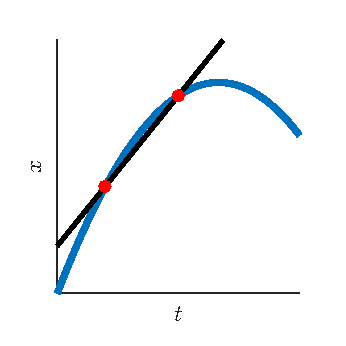
\includegraphics[width=0.3\textwidth]{Mat/matfig/gnshast.eps}
    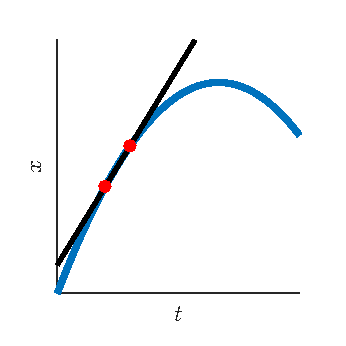
\includegraphics[width=0.3\textwidth]{Mat/matfig/gnshast2.eps}
    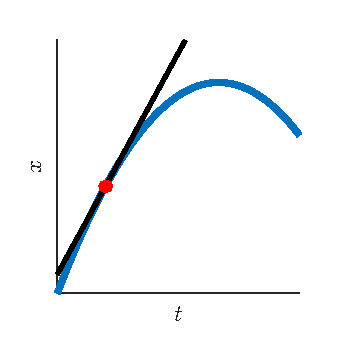
\includegraphics[width=0.3\textwidth]{Mat/matfig/hast.eps}
    \caption{Som $\Delta t$ gøres mindre vil $v_\text{gns}$ nærme sig hastigheden i punktet.}
    \label{mat:fig:diff1}
\end{figure}

Når man er ude at køre, er man normalt ikke så interesseret i, hvor hurtigt bilen har kørt over de sidste \SI{2}{km}. I stedet vil vi gerne vide, hvor hurtigt den kører i øjeblikket. I stedet for gennemsnitshastigheden over de sidste \SI{2}{km}, kan vi kigge på den over en mindre og mindre strækning, da gennemsnitshastigheden så vil komme tættere og tættere på den øjeblikkelige hastighed. Hvis vi lader den blå funktion på figur \ref{mat:fig:diff1} betegne bilens stedfunktion, så kan man se, at gennemsnitshastigheden (hældningen af den sorte linje) kommer tættere og tættere på hældningen af tangentlinjen i punktet $(t,x)$, der angiver den øjeblikkelige hastighed.  
Hvis vi bare kunne vælge det samme punkt to gange og så være færdige, ville det være dejligt, men så ender man med at dividere med nul i ligning \eqref{mat:eq:gnshast}. \emph{Man må aldrig dividere med nul}! Vi bliver altså nødt til at finde en anden måde til at bestemme hældningen af en funktion på. 

Vi må godt nok ikke dele med nul, men  vi kan gøre noget, der er næsten lige så godt. Vi kan dividere med et tal, der er så lille, at det er næsten er nul. Typisk siger man, at man dividere med noget, der er uendeligt småt, eller infinitesimalt småt, og derved kommer vi over i studiet af infinitesimalregning. Dette felt omhandler altså meget små ændringer, og deles normalt op i \emph{differentialregning} og \emph{integralregning}, to ting der har enorm betydning i fysikken.

\section{Differentialregning}
Lad os se på en funktion $f(t)$. Da er hældningen af linjen imellem to punkter $(t_1,f(t_1)$ og $(t_2,f(t_2)$, hvor $t_2 = t_1 + \Delta t$, givet ved
$$
\frac{\Delta f}{\Delta t}=\frac{f(t_2)-f(t_1)}{t_2-t_1}=\frac{f(t_1+\Delta t)-f(t_1)}{\Delta t} \, .
$$
Når vi lader $\Delta t$ nærme sig nul, vil $\Delta f/ \Delta t$ nærme sig hældningen af grafen for $f(t)$ ved tiden $t_1$. Det er det vi kalder en \emph{grænseværdi}. Grænseværdien skrives
\begin{equation} \label{mat:eq:diffkvotient}
\lim_{\Delta t\rightarrow 0}\frac{\Delta f}{\Delta t}=\dv{f}{t}=f'(t) \, .
\end{equation}
Her står $\lim$ for "limes", der er latin for grænse, men det er lettere at huske det, hvis man tænker på det engelske ord "limit". Størrelsen $\text{d}f / \text{d}t$ kaldes den \emph{differentierede} funktion\footnote{Nogle gange kaldes det også for den afledte funktion.}, og det er en ny funktion, der er forbundet med $f(t)$. Mere præcist giver $\text{d}f / \text{d}t$ os hældningen af grafen $f(t)$ til alle tider $t$ 
\footnote{Normalt skriver vi $\Delta$, når vi mener forskelle, der ikke er infinitesimale, og d når vi mener de uendeligt små forskelle.}.

Dette tillader os nu at se på øjeblikkelige hastigheder, det vi er vant til blot at kalde hastigheder. Hastigheden er altså givet som
\begin{equation}
v=\lim_{\Delta t\rightarrow 0}v_\text{gns}= \lim_{\Delta t\rightarrow 0} \frac{\Delta x}{\Delta t} = \dv{x}{t}\label{mat:eq:hast} \, .
\end{equation}
Tilsvarende til at hastighed er ændring i position over tid, så har vi også acceleration, der er ændring i hastighed over tid. Accelerationen er da 
\begin{equation}
    a=\dv{v}{t}=\dv[2]{x}{t} \, ,
\end{equation}
hvor 2-tallene angiver, at $x$ er blevet differentieret to gange.

En god ting at bemærke her er, at ligesom den første afledte af en funktion giver hældningen af funktionens graf, så giver den anden afledte krumningen af funktionens graf.
En god huskeregel til at finde fortegnet på krumningen er, at se på et lille stykke af grafen som munden af en smiley. Er smileyen glad er krumningen positiv, mens hvis smileyen er sur, er krumningen negativ\footnote{Vi ved godt at dette er en fjollet huskeregel, men ofte er de bedste huskeregler de dummeste.}.
\begin{figure}
    \centering
    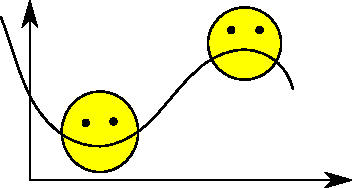
\includegraphics[width = 0.5\textwidth]{Mat/matfig/smiley.pdf}
    \caption{Illustration af krumning med smileyer. Er smileyen glad, er krumningen positiv, mens hvis smileyen er sur, er krumningen negativ.}
    \label{fig:my_label}
\end{figure}

\subsection{Om notation}
Der er to måder at angive, at man har afledte funktioner, hvilket vi kan takke Isaac  Newton og Gottfried Wilhelm Leibniz for. De opdagede nemlig infinitesimalregningen næsten samtidig.

Newton var dygtig til både matematik og fysik, men han var knap så god til at fortælle andre, hvad han havde fundet ud af. I 1666, da han var 23, havde Newton allerede udledt det matematiske grundlag til at lave differentialregning. Måden Newton skrev den afledte funktion var ved at sætte en prik ovenover, altså
$$
\dot{f}(t) \, .
$$
Det er en modifikation af denne notation, der har ført til mærkenotationen $f'(t)$, som typisk bruges i gymnasiet.

I løbet af 1670erne arbejdede tyskeren Gottfried Wilhelm Leibniz på at finde arealet under kurver, hvilket viste sig at være meget tæt forbundet med differentialregning. Leibniz offentliggjorde sit arbejde i 1684, hele to årtier før Newton endeligt offentliggjorte sit arbejde. 
Med undtagelse af nogle få breve havde Leibniz ingen adgang til Newtons arbejde med differentialregning, så han udviklede sin egen notation, hvor den afledte funktion skrives
$$
\dv{f}{t} \, .
$$
Der endte med at opstå en strid om, hvem der skulle have æren for differentialregning, og det blev afgjort af det britiske "The Royal Society"$\,$ i 1713 til fordel for Newton. At Newton var præsident for "The Royal Society"$\,$ på det tidspunkt, har efter alt sandsynlighed haft en markant effekt på denne konklusion.

Den moderne konsensus er, at Newton og Liebniz kom frem til deres resultater uafhængigt af hinanden, og derfor begge fortjener æren. Uafhængigt af hvem der var først, har Leibniznotation mange styrker, som hverken prik- eller mærkenotationen har. De er blandt andet: 
\begin{itemize}
    \item En tydelig forbindelse til hældningen.
    \item Bedre mulighed for at håndtere forskellige/flere variable.
    \item En lettere måde at differentiere flere gange.
\end{itemize}
Vi bemærker her en vigtig notation, der bruges, når man differentierer flere gange. Siden $\text{d}f / \text{d}t$ også er en funktion, er det muligt at differentiere den igen. Det skrives
\begin{equation}
    \dv{}{t}\dv{f}{t}(t)=\dv[2]{f}{t}=f''(t)=\Ddot{f}(t)\, .
\end{equation}
Den eneste praktiske anvendelse af Newtons notation findes inden for fysikken, hvor vi nogle gange skriver $\dot{f}(t)$, men \emph{kun} når vi afleder i forhold til tid. 

\subsection{Differentialregning i praksis}
Vi vil ikke gå i dybden med, hvordan man udregner afledte funktioner ud fra definitionen i ligning \eqref{mat:eq:diffkvotient}. I stedet vil vi udnytte, at langt de fleste funktioner er opbygget af nogle få simple funktioner, som er givet i tabel \ref{mat:tab:diff} sammen med deres første afledte. Bemærk at kvadratrødder og brøker kan skrives som potensfunktioner\footnote{F.eks. er $\sqrt{x} = x^{1/2}$ og $1/x = x^{-1}$.}, så disse er også indeholdt i tabellen. Ud fra tabellen og de følgende regneregler for differentialregning er det muligt af differentiere en kæmpe mængde af funktioner.
\setlength{\tabcolsep}{1.2 em}
\def\arraystretch{1.5}
\begin{table}[h!]
    \centering
    \begin{tabular}{c|c|c}
    Funktionsnavn&$f(t)$&$\dd f/\dd t$\\\specialrule{.125em}{.1em}{.1em}
    Konstant&$k$&$0$\\\hline
    Lineær funktion&$x$&$1$\\\hline
    Andengradspolynomium&$x^2$&$2x$\\\hline
    Tredjegradspolynomium&$x^3$&$3x^2$\\\hline
    Potensfunktion&$x^n$&$nx^{n-1}$\\\hline
    Sinus&$\sin(t)$&$\cos(t)$\\\hline
    Cosinus&$\cos(t)$&$-\sin(t)$\\\hline
    Tangens&$\tan(t)$&$1/\cos^2(t)$\\\hline
    Eksponentialfunktionen &$e^t$&$e^t$\\\hline
    Den naturlige logaritme & $\ln(t)$&$1/t$, hvor t > 0\\ \specialrule{.125em}{.1em}{.1em}
    \end{tabular}
    \caption{Afledte funktioner for nogle af de mest almindelige funktioner.}
    \label{mat:tab:diff}
\end{table}
%Overvej at skrive eksplicit den afledede af x x^2 x^3.
\paragraph*{Konstantreglen:} Den afledte af en funktion gange en konstant, er det samme som konstanten ganget med den afledte af funktionen:
\begin{equation}
    \dv{}{t} \left(k\cdot f(t)\right)=k\cdot\dv{f}{t}=k\cdot f'(t) \, .
\end{equation}
\paragraph*{Sumreglen:} Den afledte af summen af to funktioner, $f$ og $g$, er summen af deres afledte:
\begin{equation}
    \dv{}{t}\left(f(t)+g(t)\right)=\dv{f}{t}+\dv{g}{t}=f'(t)+g'(t) \, .
\end{equation}
\paragraph*{Differensreglen:} Kombinerer vi sumreglen med konstantreglen, får vi, at det samme gælder for differensen af to funktioner:
\begin{equation}
    \dv{}{t}\left(f(t)-g(t)\right)=\dv{f}{t}-\dv{g}{t}=f'(t)-g'(t) \, .
\end{equation}
\paragraph*{Produktreglen:} Denne regel siger, at den afledte af produktet af to funktioner er den ene funktion differentieret gange den anden udifferentieret, plus den første udifferentieret gange den anden differentieret: 
\begin{equation}
    \dv{}{t} (f(t)\cdot g(t))=f(t)\dv{g}{t}+g(t)\dv{f}{t}=f(t)g'(t)+f'(t)g(t) \, .
\end{equation}
\paragraph*{Kædereglen:} Man støder ofte på funktioner inde i andre funktioner, såkaldte sammensatte funktioner. Regnereglen for disse funktioner er:
\begin{equation}
    \dv{}{t} f\left(g(t)\right)=\dv{g}{t}\dv{f}{g}=g'(t)f'\left(g(t)\right) \, .
\end{equation}
\paragraph*{Kvotientreglen:} Der er også en regneregel for en funktion divideret med en anden:
\begin{equation}
    \dv{}{t} \frac{f(t)}{g(t)} = \frac{\dv{f}{t}g(t)-f(t)\dv{g}{t}}{g^2(t)}=\frac{f'(t)g(t)-f(t)g'(t)}{g^2(t)} \, .
\end{equation}

\subsubsection{Eksempel}
Vi vil differentiere funktionen $F(t) = (3 - t^2) e^{-t^2}$
mht. $t$. Vi starter med at betragte $F(t)$ som et produkt af to
funktioner, $3-t^2$ og $e^{-t^2}$, og bruger derfor produktregelen. Det giver at
\[
\dv{F}{t} =
\left(\dv{}{t} (3-t^2)\right) \cdot e^{-t^2}
+ (3-t^2) \cdot \left(\dv{}{t} e^{-t^2}\right)
\]
Fra tabel \ref{mat:tab:diff} kan vi se at
\[
\dv{}{t} (3-t^2) = -2t \, .
\]
Dernæst vil vi differentiere $e^{-t^2}$, som vi betragter som en
sammensat funktion. Kædereglen med $g(t) = -t^2$ og $f(g(t)) = e^{g(t)}$
giver at
\[
\dv{}{t} e^{-t^2} = \dv{}{t} (-t^2) \cdot \dv{}{g} e^g
= -2t \cdot e^g
= -2t e^{-t^2} \, .
\]
Vi kan nu samle resultaterne og beregne differentialkvotienten for $F(t)$
\[
\dv{F}{t} = (-2t) \cdot e^{-t^2} + (3-t^2) \cdot (-2t e^{-t^2})
= -2t(4 - t^2) e^{-t^2} \, .
\]